

% This is based on "sig-alternate.tex" V1.9 April 2009
% This file should be compiled with V2.4 of "sig-alternate.cls" April 2009
%
\documentclass{report}

\usepackage[english]{babel}
\usepackage{graphicx}
\usepackage{tabularx}
\usepackage{subfigure}
\usepackage{enumitem}
\usepackage{url}

\usepackage{color}
\definecolor{orange}{rgb}{1,0.5,0}
\definecolor{lightgray}{rgb}{.9,.9,.9}
\definecolor{java_keyword}{rgb}{0.37, 0.08, 0.25}
\definecolor{java_string}{rgb}{0.06, 0.10, 0.98}
\definecolor{java_comment}{rgb}{0.12, 0.38, 0.18}
\definecolor{java_doc}{rgb}{0.25,0.35,0.75}

% code listings

\usepackage{listings}
\lstloadlanguages{Java}
\lstset{
	language=Java,
	basicstyle=\scriptsize\ttfamily,
	backgroundcolor=\color{lightgray},
	keywordstyle=\color{java_keyword}\bfseries,
	stringstyle=\color{java_string},
	commentstyle=\color{java_comment},
	morecomment=[s][\color{java_doc}]{/**}{*/},
	tabsize=2,
	showtabs=false,
	extendedchars=true,
	showstringspaces=false,
	showspaces=false,
	breaklines=true,
	numbers=left,
	numberstyle=\tiny,
	numbersep=6pt,
	xleftmargin=3pt,
	xrightmargin=3pt,
	framexleftmargin=3pt,
	framexrightmargin=3pt,
	captionpos=b
}

% Disable single lines at the start of a paragraph (Schusterjungen)

\clubpenalty = 10000

% Disable single lines at the end of a paragraph (Hurenkinder)

\widowpenalty = 10000
\displaywidowpenalty = 10000
 
% allows for colored, easy-to-find todos

\newcommand{\todo}[1]{\textsf{\textbf{\textcolor{orange}{[[#1]]}}}}

% consistent references: use these instead of \label and \ref

\newcommand{\lsec}[1]{\label{sec:#1}}
\newcommand{\lssec}[1]{\label{ssec:#1}}
\newcommand{\lfig}[1]{\label{fig:#1}}
\newcommand{\ltab}[1]{\label{tab:#1}}
\newcommand{\rsec}[1]{Section~\ref{sec:#1}}
\newcommand{\rssec}[1]{Section~\ref{ssec:#1}}
\newcommand{\rfig}[1]{Figure~\ref{fig:#1}}
\newcommand{\rtab}[1]{Table~\ref{tab:#1}}
\newcommand{\rlst}[1]{Listing~\ref{#1}}

% General information

\title{Distributed Systems -- Assignment 3}

% Use the \alignauthor commands to handle the names
% and affiliations for an 'aesthetic maximum' of six authors.

\numberofauthors{3} %  in this sample file, there are a *total*
% of EIGHT authors. SIX appear on the 'first-page' (for formatting
% reasons) and the remaining two appear in the \additionalauthors section.
%
\author{
% You can go ahead and credit any number of authors here,
% e.g. one 'row of three' or two rows (consisting of one row of three
% and a second row of one, two or three).
%
% The command \alignauthor (no curly braces needed) should
% precede each author name, affiliation/snail-mail address and
% e-mail address. Additionally, tag each line of
% affiliation/address with \affaddr, and tag the
% e-mail address with \email.
%
% 1st. author
\alignauthor Robin Guldener\\
	\affaddr{ETH ID 11-930-369}\\
	\email{robing@student.ethz.ch}
% 2nd. author
\alignauthor Nico Previtali\\
	\affaddr{ETH ID 11-926-433}\\
	\email{pnico@student.ethz.ch}
%% 3rd. author
\alignauthor Lukas Bischofbergeryxcvyxcvxyv\\
	\affaddr{ETH ID 11-915-907}\\
	\email{lukasbi@student.ethz.ch}
%\and  % use '\and' if you need 'another row' of author names
%% 4th. author
%\alignauthor Student Four\\
% 	\affaddr{ETH ID XX-XXX-XXX}\\
% 	\email{four@student.ethz.ch}
%% 5th. author
%\alignauthor Student Five\\
% 	\affaddr{ETH ID XX-XXX-XXX}\\
% 	\email{five@student.ethz.ch}
%% 6th. author
%\alignauthor Student Six\\
% 	\affaddr{ETH ID XX-XXX-XXX}\\
% 	\email{six@student.ethz.ch}
}


\begin{document}

\maketitle

\begin{abstract}
For the implementation of this assignment we made use of the two lab provided HTC desire number 25 and 37 and a private Samsung Galaxy Tab 2. We were able to implement both assignments and to our best knowledge both chats are working flawlessly. 
%Concisely state (i) which Android device you used, (ii) which tasks you completed and which are working correctly or limited, and (iii) what your specific enhancements are.
\end{abstract}

\section{Introduction}

%Use the introduction for background information on the assignment.
\begin{itemize}
  \item Lamport timestamps\cite{lamport} and vector clocks\cite{vector_clocks} are used to order the messages we receive from the chat server. Both timestamps are stored for all messages implicitly since we always store the entire JSONObject returned from the server. This has the advantage that large parts of our chat implementation is shared between the lamport and the vector clock version, which eases maintenance and sped up our development process. For Lamport timestamps we explicitly ordered the messages as they were arriving whereas for vector clocks we only order the messages implicitly in the displaying ListView. Further details regarding these implementations can be found in the respective sections below.%Please give an overview of the usage of the Lamport times and of the Vector Clocks.
  \item %Also write about your architecture to handle the UDP communication.
  We used asynchronous tasks to register, unregister, get clients/server information from the server and sending chat messages. So these tasks can send and possibly also receive packets. For receiving information from the server, e.g chat messages and logout information about other clients we have implemented a background thread which has only the purpose to listen for incoming UDP packets. 
\end{itemize}

\section{Lamport Timestamps}

\begin{figure}
    \centering
    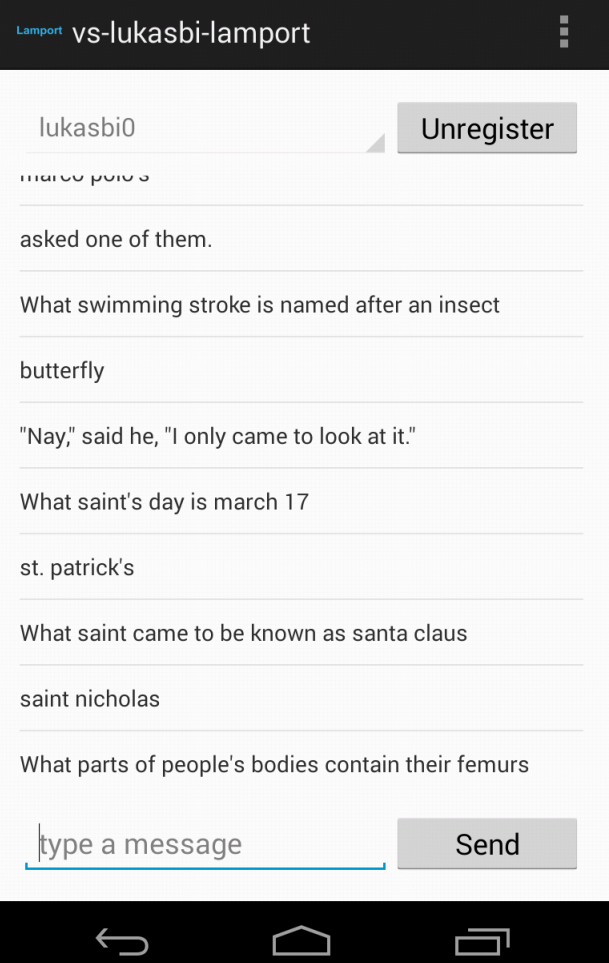
\includegraphics[height=4.2cm]{lamport.png}
    \lfig{axis}   
    \caption{Lamport Chat overview}
\end{figure}
\begin{itemize}
  
  %\item Describe shortly, how you designed your application to implement this task. Include 1-2 screenshots of your app.
  \item The UI thread has a field called \texttt{lamportTime} which stores the current Timestamps for this process. When recieving a new message the Lamport Timestamp is updated according to the algorithm presented in the lecture. When sending a new message the current Lamport Timestamp of the process is attached to the JSON object and then sent to the chat server.
  %\item Highlight the backbone of your implementation (methods) and add a state transition diagram to describe the logic behind the handling of communication with the server. Especially, describe how you designed the \texttt{isDeliverable(...)} method.
  \item For all commands that are being sent to the chat server we provide a AsyncTask which then communicates in the background with the chat server. This AsyncTask \cite{androidAsyncTask} is reserved for all outgoing UDP packets. On the other side we implemented functionality to only recieve UDP packets. This class (providing the mentioned functionality) is running in a seperate thread and its main goal is to catch all incoming chat messages and the server status. The recieved messages are then sent to the UI thread for displaying them. This is done with the use of an Handler \cite{androidHandler}. For better understanding see the state transition diagram (cf. \rfig{std}).
  %\item Describe the main problem encountered in this task and give an overview of your solution.
  \item The main problem was that we first tried to connected to the same UDP Port which is obviously not possible.
\end{itemize}

\begin{figure}
    \centering
    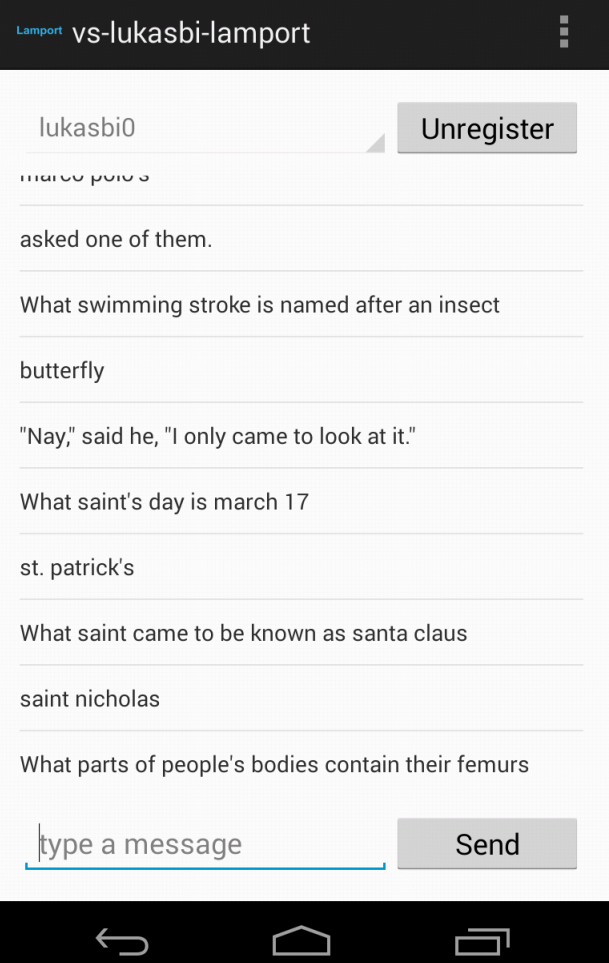
\includegraphics[height=4.2cm]{std.png}
    \lfig{std}   
    \caption{State transition diagram}
\end{figure}

\section{Vector Clocks}
\begin{itemize}
  %\item Did you reuse elements from Task 2? Highlight the main differences to Task 2.
  \item To achieve efficiency we reused the whole code of Task 2. The main differences are that we now implemented Vector clocks and discarded Lamport Timestamps. For this we had do change the handler to parse the recieved JSON to extract and build the vector clock. Another main difference is that we introduced a new class called \texttt{VectorClockComparator} which is able to compare two vector clock timestamps.

\lstset{language=Java,caption={Using AsyncTask},label=asynctask} 
\begin{lstlisting}
public class VectorClockComparator implements Comparator<JSONObject> {
	@Override
	/**
     * o1 is before o2 iff both conditions are met:
     * - each process's clock is less-than-or-equal-to its own clock in other; and
     * - there is at least one process's clock which is strictly less-than its
     *   own clock in o2
     */
    public int compare(JSONObject o1, JSONObject o2) {
		int isBefore = 0;
		
		// Since we are not guaranteed that both objects have the same indexes compute intersection and compare based on that
		HashMap<String, Integer> vector1 = MainActivity.vectorClockFromJSON(o1);
		HashMap<String, Integer> vector2 = MainActivity.vectorClockFromJSON(o2);
		HashMap<String, Integer> intersection = new HashMap<String, Integer>(vector1);
		intersection.keySet().retainAll(vector2.keySet());
		
		for (String key : intersection.keySet()) {
			int val1 = vector1.get(key);
			int val2 = vector2.get(key);
			
			if (val1 > val2)
				return 1;
			else if (val1 < val2)
				isBefore = -1;
			
		}
		
		return isBefore;
	}
}
\end{lstlisting}
  \item Since we cannot reliably compare two vector clocks with this chat implementation (this is due to the fact that the number of objects in the clock and the devices they represent may vary from message to message) we were unsure how to reliably order vector clock messages and guarantee direct consecutive ordering. This also represented our main challenge in this part of the application and since we could not come up with a satisfactory definition for consecutive ordering we finally agreed in ignoring the isDeliverable method and to provide at best-effor total ordering of the incoming messages. This is also reflected in our comparator listed above, which makes use of the intersection to order any two messages but this is not ideal from a theoretical standpoint and may not always yield good absolute orders. Further information regarding vector clocks from the lecture would have been beneficial.
\end{itemize}

\section{Discussion}
Please reply to the following questions.
\begin{itemize}
  \item \textbf{What are the main advantages of using Vector Clocks over Lamport Timestamps?} The system of vector clocks is strongly consistent. Thus, by comparing the vector timestamp of two events, we can determine if the events are causally related. This is called the \textit{strong clock consistency condition}. Using only a Lamport Timestamps, only a partial causal ordering can be inferred from the clock (the implication goes only in one way, called the \textit{clock consistency condition}).
  \item \textbf{When exactly are two Vector Clocks causally dependent?} The conditions are already listed in the code snippet but are repeated here. For two vector clocks to be causally dependent they need to be either each clock in the first is less than or equal to the clocks in the second OR there is at least one clock in process one that is strictly less than it's own clock in the second.
  \item \textbf{Does a clock tick happen before or after the sending of a message. What are the implications of changing this?} We decided that we would not let our applications trigger a tick when receiving a message. The implications of also ticking the clock on a message receive would be that consecutive ordering could no longer be guaranteed, since it is not known how many messages any client received before sending the next one.
  \item \textbf{Read and assess the paper Tobias Landes - Dynamic Vector Clocks for Consistent Ordering of Events in Dynamic Distributed Applications3 that gives a good overview on the discussed methods. In particular, which problem of vector clocks is solved in the paper?} The paper investigates the implications of dynamic arriving and leaving of processes on the vector clock logical time ordering system. Whilst the original vector clocks are not sufficient for such situation, the paper presents a workable solution for such dynamic environements that builds on the original vector clocks idea and extends the known concept.
\end{itemize}


\section{Conclusion}

%Give an overall conclusion that summarizes the main challenges you encountered, your lessons learned and how you divided the work load in your team.
One main challenge we encountered was to make two threads listening to the same UDP port. We first tried to handle this by sending and retrieving all commands and messages through the same thread. But then we decided to handle this challenge by binding one of the two threads to the current used port rather than just using one thread. We did it this way because then we can seperate between just listening to a UDP port for incoming messages (the chat and status messages) and sending commands to the chat server (such as deregister or sending a message). We think this is a much better design style especially when someone tries to read and understand our code.

To achieve good efficiency we divided the work into three seperate parts. Each team member worked on one part. Because the parts may overlapped we worked sometimes in parallel and sometimes not. The first part consisted of the following tasks
\begin{itemize}
  \item Setup up the whole UI and provide each UI element with the related functionality. 
  \item Setup up an AsyncTask for register / deregister commands as well as for retrieving the server status and a client list.
  \item Design the basic layout and functionality of the UDP listener thread. The UDP listener is design to be able to communicate with the UI thread because message have to be passed from the UDP listener thread to the UI.
\end{itemize}

% lukas
The second part consisted of
\begin{itemize}
  \item 1
  \item 2
  \item 3
\end{itemize}

%robin
Last we had to
\begin{itemize}
  \item Implement the \texttt{ChatAdapter} for dynamicly populating the ListView
  \item Implement the isDeliverable method for lamport timestamps and cache all incoming requests until all consecutive messages arrived
  \item Implement the vector clocks comparator and figure out how to order two messages with different vector clock entries
\end{itemize}
% The following two commands are all you need in the
% initial runs of your .tex file to
% produce the bibliography for the citations in your paper.
\bibliographystyle{abbrv}
\bibliography{report}  % sigproc.bib is the name of the Bibliography in this case
% You must have a proper ".bib" file

%\balancecolumns % GM June 2007

\end{document}
